\documentclass{ximera}

%\usepackage{todonotes}

\newcommand{\todo}{}

\usepackage{esint} % for \oiint
\ifxake%%https://math.meta.stackexchange.com/questions/9973/how-do-you-render-a-closed-surface-double-integral
\renewcommand{\oiint}{{\large\bigcirc}\kern-1.56em\iint}
\fi


\graphicspath{
  {./}
  {ximeraTutorial/}
  {basicPhilosophy/}
  {functionsOfSeveralVariables/}
  {normalVectors/}
  {lagrangeMultipliers/}
  {vectorFields/}
  {greensTheorem/}
  {shapeOfThingsToCome/}
  {dotProducts/}
  {partialDerivativesAndTheGradientVector/}
  {../productAndQuotientRules/exercises/}
  {../normalVectors/exercisesParametricPlots/}
  {../continuityOfFunctionsOfSeveralVariables/exercises/}
  {../partialDerivativesAndTheGradientVector/exercises/}
  {../directionalDerivativeAndChainRule/exercises/}
  {../commonCoordinates/exercisesCylindricalCoordinates/}
  {../commonCoordinates/exercisesSphericalCoordinates/}
  {../greensTheorem/exercisesCurlAndLineIntegrals/}
  {../greensTheorem/exercisesDivergenceAndLineIntegrals/}
  {../shapeOfThingsToCome/exercisesDivergenceTheorem/}
  {../greensTheorem/}
  {../shapeOfThingsToCome/}
  {../separableDifferentialEquations/exercises/}
  {vectorFields/}
}

\newcommand{\mooculus}{\textsf{\textbf{MOOC}\textnormal{\textsf{ULUS}}}}

\usepackage{tkz-euclide}
\usepackage{tikz}
\usepackage{tikz-cd}
\usetikzlibrary{arrows}
\tikzset{>=stealth,commutative diagrams/.cd,
  arrow style=tikz,diagrams={>=stealth}} %% cool arrow head
\tikzset{shorten <>/.style={ shorten >=#1, shorten <=#1 } } %% allows shorter vectors

\usetikzlibrary{backgrounds} %% for boxes around graphs
\usetikzlibrary{shapes,positioning}  %% Clouds and stars
\usetikzlibrary{matrix} %% for matrix
\usepgfplotslibrary{polar} %% for polar plots
\usepgfplotslibrary{fillbetween} %% to shade area between curves in TikZ
%\usetkzobj{all}
\usepackage[makeroom]{cancel} %% for strike outs
%\usepackage{mathtools} %% for pretty underbrace % Breaks Ximera
%\usepackage{multicol}
\usepackage{pgffor} %% required for integral for loops



%% http://tex.stackexchange.com/questions/66490/drawing-a-tikz-arc-specifying-the-center
%% Draws beach ball
\tikzset{pics/carc/.style args={#1:#2:#3}{code={\draw[pic actions] (#1:#3) arc(#1:#2:#3);}}}



\usepackage{array}
\setlength{\extrarowheight}{+.1cm}
\newdimen\digitwidth
\settowidth\digitwidth{9}
\def\divrule#1#2{
\noalign{\moveright#1\digitwidth
\vbox{\hrule width#2\digitwidth}}}




% \newcommand{\RR}{\mathbb R}
% \newcommand{\R}{\mathbb R}
% \newcommand{\N}{\mathbb N}
% \newcommand{\Z}{\mathbb Z}

\newcommand{\sagemath}{\textsf{SageMath}}


%\renewcommand{\d}{\,d\!}
%\renewcommand{\d}{\mathop{}\!d}
%\newcommand{\dd}[2][]{\frac{\d #1}{\d #2}}
%\newcommand{\pp}[2][]{\frac{\partial #1}{\partial #2}}
% \renewcommand{\l}{\ell}
%\newcommand{\ddx}{\frac{d}{\d x}}

% \newcommand{\zeroOverZero}{\ensuremath{\boldsymbol{\tfrac{0}{0}}}}
%\newcommand{\inftyOverInfty}{\ensuremath{\boldsymbol{\tfrac{\infty}{\infty}}}}
%\newcommand{\zeroOverInfty}{\ensuremath{\boldsymbol{\tfrac{0}{\infty}}}}
%\newcommand{\zeroTimesInfty}{\ensuremath{\small\boldsymbol{0\cdot \infty}}}
%\newcommand{\inftyMinusInfty}{\ensuremath{\small\boldsymbol{\infty - \infty}}}
%\newcommand{\oneToInfty}{\ensuremath{\boldsymbol{1^\infty}}}
%\newcommand{\zeroToZero}{\ensuremath{\boldsymbol{0^0}}}
%\newcommand{\inftyToZero}{\ensuremath{\boldsymbol{\infty^0}}}



% \newcommand{\numOverZero}{\ensuremath{\boldsymbol{\tfrac{\#}{0}}}}
% \newcommand{\dfn}{\textbf}
% \newcommand{\unit}{\,\mathrm}
% \newcommand{\unit}{\mathop{}\!\mathrm}
% \newcommand{\eval}[1]{\bigg[ #1 \bigg]}
% \newcommand{\seq}[1]{\left( #1 \right)}
% \renewcommand{\epsilon}{\varepsilon}
% \renewcommand{\phi}{\varphi}


% \renewcommand{\iff}{\Leftrightarrow}

% \DeclareMathOperator{\arccot}{arccot}
% \DeclareMathOperator{\arcsec}{arcsec}
% \DeclareMathOperator{\arccsc}{arccsc}
% \DeclareMathOperator{\si}{Si}
% \DeclareMathOperator{\scal}{scal}
% \DeclareMathOperator{\sign}{sign}


%% \newcommand{\tightoverset}[2]{% for arrow vec
%%   \mathop{#2}\limits^{\vbox to -.5ex{\kern-0.75ex\hbox{$#1$}\vss}}}
% \newcommand{\arrowvec}[1]{{\overset{\rightharpoonup}{#1}}}
% \renewcommand{\vec}[1]{\arrowvec{\mathbf{#1}}}
% \renewcommand{\vec}[1]{{\overset{\boldsymbol{\rightharpoonup}}{\mathbf{#1}}}}

% \newcommand{\point}[1]{\left(#1\right)} %this allows \vector{ to be changed to \vector{ with a quick find and replace
% \newcommand{\pt}[1]{\mathbf{#1}} %this allows \vec{ to be changed to \vec{ with a quick find and replace
% \newcommand{\Lim}[2]{\lim_{\point{#1} \to \point{#2}}} %Bart, I changed this to point since I want to use it.  It runs through both of the exercise and exerciseE files in limits section, which is why it was in each document to start with.

% \DeclareMathOperator{\proj}{\mathbf{proj}}
% \newcommand{\veci}{{\boldsymbol{\hat{\imath}}}}
% \newcommand{\vecj}{{\boldsymbol{\hat{\jmath}}}}
% \newcommand{\veck}{{\boldsymbol{\hat{k}}}}
% \newcommand{\vecl}{\vec{\boldsymbol{\l}}}
% \newcommand{\uvec}[1]{\mathbf{\hat{#1}}}
% \newcommand{\utan}{\mathbf{\hat{t}}}
% \newcommand{\unormal}{\mathbf{\hat{n}}}
% \newcommand{\ubinormal}{\mathbf{\hat{b}}}

% \newcommand{\dotp}{\bullet}
% \newcommand{\cross}{\boldsymbol\times}
% \newcommand{\grad}{\boldsymbol\nabla}
% \newcommand{\divergence}{\grad\dotp}
% \newcommand{\curl}{\grad\cross}
%\DeclareMathOperator{\divergence}{divergence}
%\DeclareMathOperator{\curl}[1]{\grad\cross #1}
% \newcommand{\lto}{\mathop{\longrightarrow\,}\limits}

% \renewcommand{\bar}{\overline}

\colorlet{textColor}{black}
\colorlet{background}{white}
\colorlet{penColor}{blue!50!black} % Color of a curve in a plot
\colorlet{penColor2}{red!50!black}% Color of a curve in a plot
\colorlet{penColor3}{red!50!blue} % Color of a curve in a plot
\colorlet{penColor4}{green!50!black} % Color of a curve in a plot
\colorlet{penColor5}{orange!80!black} % Color of a curve in a plot
\colorlet{penColor6}{yellow!70!black} % Color of a curve in a plot
\colorlet{fill1}{penColor!20} % Color of fill in a plot
\colorlet{fill2}{penColor2!20} % Color of fill in a plot
\colorlet{fillp}{fill1} % Color of positive area
\colorlet{filln}{penColor2!20} % Color of negative area
\colorlet{fill3}{penColor3!20} % Fill
\colorlet{fill4}{penColor4!20} % Fill
\colorlet{fill5}{penColor5!20} % Fill
\colorlet{gridColor}{gray!50} % Color of grid in a plot

\newcommand{\surfaceColor}{violet}
\newcommand{\surfaceColorTwo}{redyellow}
\newcommand{\sliceColor}{greenyellow}




\pgfmathdeclarefunction{gauss}{2}{% gives gaussian
  \pgfmathparse{1/(#2*sqrt(2*pi))*exp(-((x-#1)^2)/(2*#2^2))}%
}


%%%%%%%%%%%%%
%% Vectors
%%%%%%%%%%%%%

%% Simple horiz vectors
\renewcommand{\vector}[1]{\left\langle #1\right\rangle}


%% %% Complex Horiz Vectors with angle brackets
%% \makeatletter
%% \renewcommand{\vector}[2][ , ]{\left\langle%
%%   \def\nextitem{\def\nextitem{#1}}%
%%   \@for \el:=#2\do{\nextitem\el}\right\rangle%
%% }
%% \makeatother

%% %% Vertical Vectors
%% \def\vector#1{\begin{bmatrix}\vecListA#1,,\end{bmatrix}}
%% \def\vecListA#1,{\if,#1,\else #1\cr \expandafter \vecListA \fi}

%%%%%%%%%%%%%
%% End of vectors
%%%%%%%%%%%%%

%\newcommand{\fullwidth}{}
%\newcommand{\normalwidth}{}



%% makes a snazzy t-chart for evaluating functions
%\newenvironment{tchart}{\rowcolors{2}{}{background!90!textColor}\array}{\endarray}

%%This is to help with formatting on future title pages.
\newenvironment{sectionOutcomes}{}{}



%% Flowchart stuff
%\tikzstyle{startstop} = [rectangle, rounded corners, minimum width=3cm, minimum height=1cm,text centered, draw=black]
%\tikzstyle{question} = [rectangle, minimum width=3cm, minimum height=1cm, text centered, draw=black]
%\tikzstyle{decision} = [trapezium, trapezium left angle=70, trapezium right angle=110, minimum width=3cm, minimum height=1cm, text centered, draw=black]
%\tikzstyle{question} = [rectangle, rounded corners, minimum width=3cm, minimum height=1cm,text centered, draw=black]
%\tikzstyle{process} = [rectangle, minimum width=3cm, minimum height=1cm, text centered, draw=black]
%\tikzstyle{decision} = [trapezium, trapezium left angle=70, trapezium right angle=110, minimum width=3cm, minimum height=1cm, text centered, draw=black]


\title{Theory}

\begin{document}

\begin{abstract}
the quadratic story
\end{abstract}
\maketitle




We have investigated quadratic functions from several viewpoints.  Time to collect all of our thoughts and characterize quadratic functions.





\begin{definition} \textbf{\textcolor{green!50!black}{Quadratic Functions}} 


A \textbf{quadratic function} is a function that can be represented by a formula of the form


\[   Q(t) = a \, t^2 + b \, t + c         \]

where $a$, $b$, $c$ are real numbers and $a \ne 0$.


\end{definition}



$\blacktriangleright$ \textbf{\textcolor{red!10!blue!90!}{Domain:}} \\

The natural or implied domain of a quadratic function is all real numbers.  Of course, a particular quadratic function may be defined with a subset of the real numbers.  We may refer to these as \textbf{restricted} quadratic functions.






\begin{formula} \textbf{\textcolor{purple!85!blue}{Forms}}

Formulas for quadratic functions have three basic forms:



\begin{itemize}
\item \textbf{\textcolor{purple!85!blue}{Standard Form:}}  The standard form for a quadratic function looks like a sum of terms
\[ a \, t^2 + b \, t + c \]
\item \textbf{\textcolor{purple!85!blue}{Factored Form:}}  The factored form for a quadratic function looks like a product of factors
\[ a(t - r_1)(t - r_2) \]
\item \textbf{\textcolor{purple!85!blue}{Vertex Form:}}  The vertex form for a quadratic function looks like 
\[ a(t - h)^2 + k \]
\end{itemize}



Each form serves a different purpose.  For analysis purposes, the factored form reveals the zeros of the quadratic function and the vertex form reveals the extreme value of the function.


\end{formula}

\textbf{Note:} So far, we have restricted our investigation to quadratics with real roots (or zeros).  Therefore, we encounter quadratics that do not factor for us with real numbers. We call these \textbf{irreducible quadratics}.  Later, in this course, we will bring in complex numbers and complete our characterization of quadratic functions. Complex numbers will allow us to factor all quadratics.




\begin{notation} 

In the standard form $Q(t) = a \, t^2 + b \, t + c  $,


\begin{itemize}
\item $a \, t^2$ is called the \textbf{leading term}
\item $a$ is called the \textbf{leading coefficient}
\item $b \, t$ is called the \textbf{linear term}
\item $b$ is called the \textbf{linear coefficient}
\item $c$ is called the \textbf{constant term}
\end{itemize}





\end{notation}





$\blacktriangleright$ \textbf{\textcolor{red!10!blue!90!}{Graph}} \\ 

The graph of a quadratic function is a parabola, which opens up or down.  The direction depends on the sign of the leading coefficient, $a$.








\begin{image}
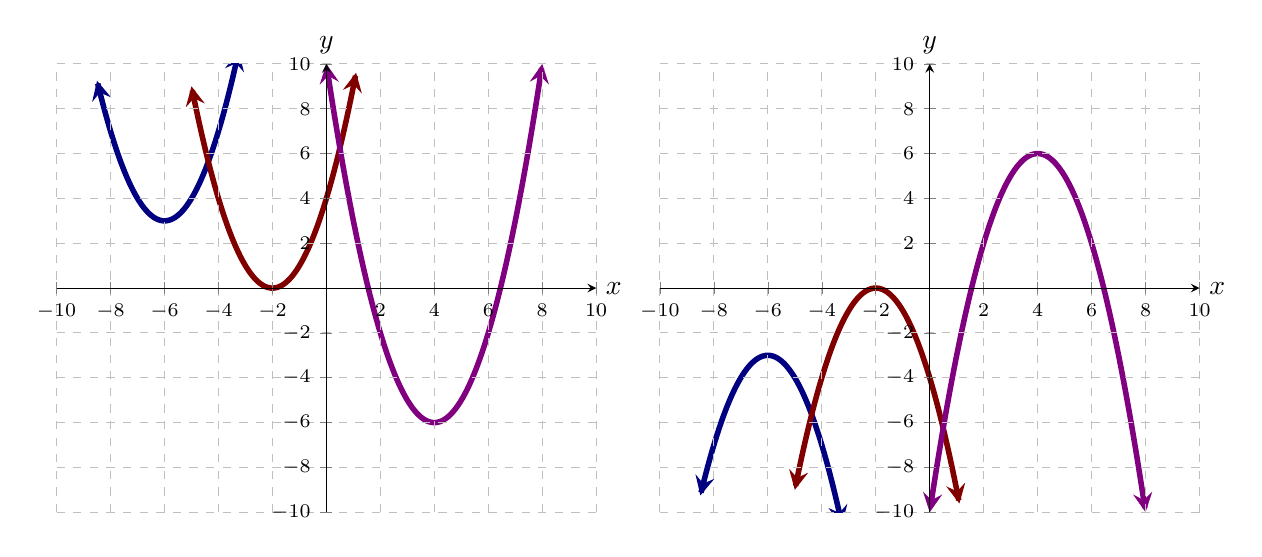
\begin{tikzpicture}
  \begin{axis}[name = leftgraph,
            domain=-10:10, ymax=10, xmax=10, ymin=-10, xmin=-10,
            axis lines =center, xlabel=$x$, ylabel=$y$, grid = major, grid style={dashed},
            ytick={-10,-8,-6,-4,-2,2,4,6,8,10},
            xtick={-10,-8,-6,-4,-2,2,4,6,8,10},
            yticklabels={$-10$,$-8$,$-6$,$-4$,$-2$,$2$,$4$,$6$,$8$,$10$}, 
            xticklabels={$-10$,$-8$,$-6$,$-4$,$-2$,$2$,$4$,$6$,$8$,$10$},
            ticklabel style={font=\scriptsize},
            every axis y label/.style={at=(current axis.above origin),anchor=south},
            every axis x label/.style={at=(current axis.right of origin),anchor=west},
            axis on top
          ]
          

            \addplot [line width=2, penColor, smooth,samples=200,domain=(-8.5:-3.25),<->] {(x+6)^2+3};
            \addplot [line width=2, penColor2, smooth,samples=200,domain=(-5:1.1),<->] {(x+2)^2};
            \addplot [line width=2, penColor3, smooth,samples=200,domain=(0:8),<->] {(x-4)^2-6};



           

  \end{axis}
  \begin{axis}[at={(leftgraph.outer east)},anchor=outer west,
            domain=-10:10, ymax=10, xmax=10, ymin=-10, xmin=-10,
            axis lines =center, xlabel=$x$, ylabel=$y$, grid = major, grid style={dashed},
            ytick={-10,-8,-6,-4,-2,2,4,6,8,10},
            xtick={-10,-8,-6,-4,-2,2,4,6,8,10},
            yticklabels={$-10$,$-8$,$-6$,$-4$,$-2$,$2$,$4$,$6$,$8$,$10$}, 
            xticklabels={$-10$,$-8$,$-6$,$-4$,$-2$,$2$,$4$,$6$,$8$,$10$},
            ticklabel style={font=\scriptsize},
            every axis y label/.style={at=(current axis.above origin),anchor=south},
            every axis x label/.style={at=(current axis.right of origin),anchor=west},
            axis on top
          ]
          
			\addplot [line width=2, penColor, smooth,samples=200,domain=(-8.5:-3.25),<->] {-(x+6)^2-3};
            \addplot [line width=2, penColor2, smooth,samples=200,domain=(-5:1.1),<->] {-(x+2)^2};
            \addplot [line width=2, penColor3, smooth,samples=200,domain=(0:8),<->] {-(x-4)^2+6};


           

  \end{axis}
\end{tikzpicture}
\end{image}





$\blacktriangleright$ \textbf{\textcolor{red!10!blue!90!}{Zeros (1)}} \\
Quadratic functions always have two roots.  However, these roots can be complex numbers, which we will encounter later in this course.  Restricting ourselves to only real numbers means that our quadratics have $0$, $1$, or $2$ real roots.  These correspond to  $0$, $1$, or $2$ intercepts on the graph, which correspond to $0$, $1$, or $2$ distinct factors over the real numbers. 

Quadratics are a type of polynomial and zeros of polynomials are also called \textbf{roots}.

\begin{itemize}
\item The two roots can be different (distinct) numbers corresponding to two different factors and intercepts on the graph.  
\item The two roots can be the same number.  In this case, the factorization is a square: $Q(t) = a(t-r)^2$.  The root has an even multiplicity and the vertex of the parabola is the single intercept.
\item The two roots can both be complex numbers.  There are no real roots. There are no intercepts on the graph. The quadratic does not factor over the real numbers.
\end{itemize}


$\blacktriangleright$ \textbf{\textcolor{red!10!blue!90!}{Range}} \\
From the graphs, we can see that the there are two types of ranges: 
\begin{itemize}
\item $(-\infty, k]$ if the leading coefficient is negative and the parabola opens down.
\item $[k, \infty)$ if the leading coefficient is positive and the parabola opens up.
\end{itemize}

$k$ is the constant term in the vertex form.



$\blacktriangleright$  \textbf{\textcolor{red!10!blue!90!}{Extrema}} \\
From the graphs, we can see that there are two situations:
\begin{itemize}
\item The function has a single maximum value of $k$, if the leading coefficient is negative. The parabola opens down.
\item The function has a single minimum value of $k$, if the leading coefficient is positive. The parabola opens up.
\end{itemize}

$k$ is the constant term in the vertex form.




$\blacktriangleright$ \textbf{\textcolor{red!10!blue!90!}{Rate-of-Change}} \\
\begin{itemize}
\item If the leading coefficient is negative and the parabola opens down, then the function increases on $(-\infty, h]$ and decreases on $[h, \infty)$, where $h$ is from the vertex form.
\item If the leading coefficient is positive and the parabola opens up, then the function decreases on $(-\infty, h]$ and increases on $[h, \infty)$, where $h$ is from the vertex form.
\end{itemize}





$\blacktriangleright$ \textbf{\textcolor{red!10!blue!90!}{Axis of Symmetry}} \\ 
The vertex form, $Q(t) = a(t-h)^2 + k$ shows us that the graph is symmetric about the vertical line, $t=h$.  This is the line of symmetry or the axis of symmetry.  This should be drawn on the graph.

















\begin{image}
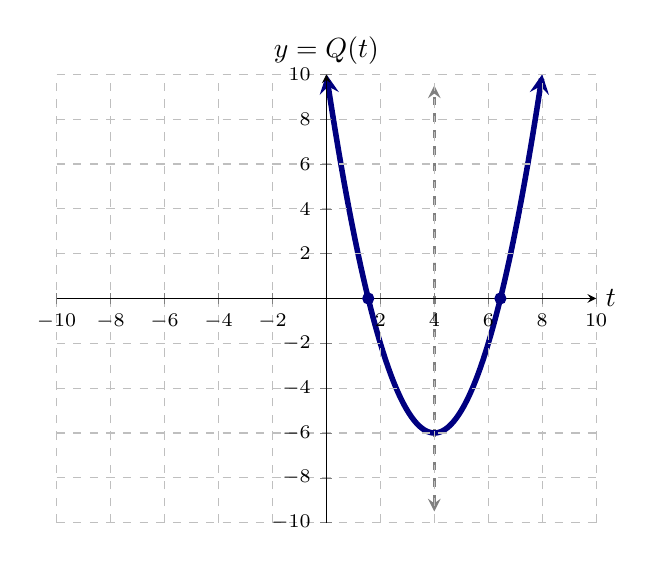
\begin{tikzpicture}
  \begin{axis}[
            domain=-10:10, ymax=10, xmax=10, ymin=-10, xmin=-10,
            axis lines =center, xlabel=$t$, ylabel={$y=Q(t)$}, grid = major, grid style={dashed},
            ytick={-10,-8,-6,-4,-2,2,4,6,8,10},
            xtick={-10,-8,-6,-4,-2,2,4,6,8,10},
            yticklabels={$-10$,$-8$,$-6$,$-4$,$-2$,$2$,$4$,$6$,$8$,$10$}, 
            xticklabels={$-10$,$-8$,$-6$,$-4$,$-2$,$2$,$4$,$6$,$8$,$10$},
            ticklabel style={font=\scriptsize},
            every axis y label/.style={at=(current axis.above origin),anchor=south},
            every axis x label/.style={at=(current axis.right of origin),anchor=west},
            axis on top
          ]
          

			\addplot [line width=1, gray, dashed, domain=(-9.5:9.5),<->] ({4},{x});
			\addplot [line width=2, penColor, smooth,samples=200,domain=(0:8),<->] {(x-4)^2 - 6};

          %\addplot[color=penColor,fill=penColor2,only marks,mark=*] coordinates{(-6,9)};
          %\addplot[color=penColor,fill=penColor2,only marks,mark=*] coordinates{(2,-7)};

			\addplot[color=penColor,fill=penColor,only marks,mark=*] coordinates{(1.551,0)};
			\addplot[color=penColor,fill=penColor,only marks,mark=*] coordinates{(6.449,0)};


           

  \end{axis}
\end{tikzpicture}
\end{image}






$\blacktriangleright$ \textbf{\textcolor{red!10!blue!90!}{Zeros (2)}} \\ 
Our quadratic functions have $0$, $1$, or $2$ real roots or zeros.  These can be obtained from any of the three forms.


\begin{itemize}

\item \textbf{\textcolor{purple!85!blue}{Standard Form:}}  Given the standard form, $Q(t) = a \, t^2 + b \, t + c$, we can use the \textbf{Quadratic Formula}.

The zeros of $Q(t) = a \, t^2 + b \, t + c$ are

\[   \frac{-b + \sqrt{b^2 - 4 \, a \, c}}{2a}      \, \text{ and } \,       \frac{-b - \sqrt{b^2 - 4 \, a \, c}}{2a}    \]



$b^2 - 4 \, a \, c$ is known as the \textbf{discriminant}. 




\begin{itemize}
\item If $b^2 - 4 \, a \, c > 0$, then there are two real zeros.
\item If $b^2 - 4 \, a \, c = 0$, then there is one real zero, because the square root will be $0$.
\item If $b^2 - 4 \, a \, c < 0$, then there are no real zeros.  They will be complex numbers.
\end{itemize}





\item \textbf{\textcolor{purple!85!blue}{Factored Form:}} \\ 
Given the factored form, $Q(t) = a (t - r_1)(t - r_2)$, we can read off the roots or zeros as $r_1$ and $r_2$. Many times the leading coefficient, $a$, is not factored out.  The zero product property allows us to set each factor equal to $0$ and solve.






\item  \textbf{\textcolor{purple!85!blue}{Vertex Form:}} \\
Given the vertex form, $Q(t) = a (t - h)^2 + k$, we can set the formula equal to $0$ and solve.



\begin{align*}
a (t - h)^2 + k    & = 0  \\
a (t - h)^2        & = -k  \\
(t - h)^2        & = -\frac{k}{a}  \\
t - h        & = \pm \sqrt{-\frac{k}{a}}  \\
t        & = \pm \sqrt{-\frac{k}{a}}  + h
\end{align*}

From $a (t - h)^2 + k  = 0$, we can see that if $a$ and $k$ have the same sign, then there are no real solutions.  The zeros are complex numbers.



\end{itemize}



\begin{observation}



From the vertex form, we see that the zeros or roots include the term $\sqrt{-\frac{k}{a}}$.  The inside of the square root is $-\frac{k}{a}$.  This inside is negative if $a$ and $k$ have the same sign. This inside is positive if $a$ and $k$ have opposite sign. \\

There are real roots when $a$ and $k$ have opposite sign in vertex form. \\



\end{observation}





























\begin{example}  Quadratic Analysis



Analyze $M(t) = -\frac{1}{2} (t-3)^2 + 5$ \\


\begin{explanation}

$M$ is a quadratic function, which means its graph is a parabola.  The leading coefficient is negative, which means the parabola is opening down.  The highest point on the parabola is $(3, 5)$. From this, we know there are two intercepts, which means two roots and two factors.






\begin{image}
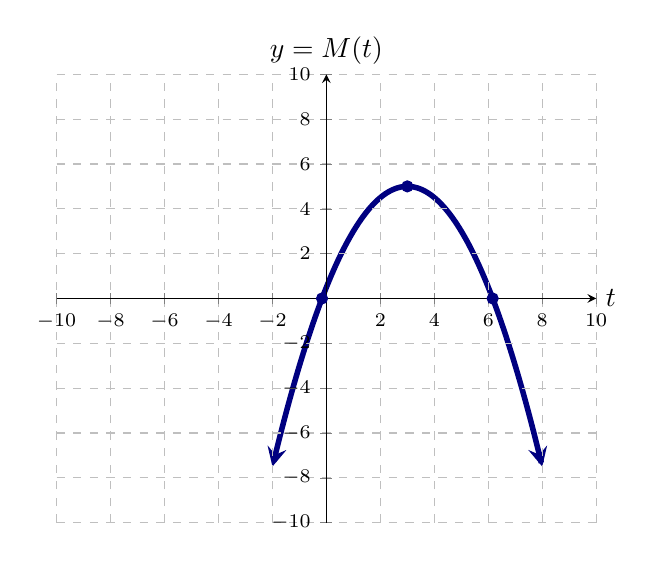
\begin{tikzpicture}
  \begin{axis}[
            domain=-10:10, ymax=10, xmax=10, ymin=-10, xmin=-10,
            axis lines =center, xlabel=$t$, ylabel={$y=M(t)$}, grid = major, grid style={dashed},
            ytick={-10,-8,-6,-4,-2,2,4,6,8,10},
            xtick={-10,-8,-6,-4,-2,2,4,6,8,10},
            yticklabels={$-10$,$-8$,$-6$,$-4$,$-2$,$2$,$4$,$6$,$8$,$10$}, 
            xticklabels={$-10$,$-8$,$-6$,$-4$,$-2$,$2$,$4$,$6$,$8$,$10$},
            ticklabel style={font=\scriptsize},
            every axis y label/.style={at=(current axis.above origin),anchor=south},
            every axis x label/.style={at=(current axis.right of origin),anchor=west},
            axis on top
          ]
          
          %\addplot [line width=2, penColor2, smooth,samples=100,domain=(-6:2)] {-2*x-3};
          \addplot [line width=2, penColor, smooth,samples=200,domain=(-2:8),<->] {-0.5*(x-3)^2 + 5};
          %\addplot [line width=2, penColor, smooth,samples=200,domain=(-7:-4),<-] {-e^(-x-5)};

          %\addplot[color=penColor,fill=penColor2,only marks,mark=*] coordinates{(-6,9)};
          %\addplot[color=penColor,fill=penColor2,only marks,mark=*] coordinates{(2,-7)};

          \addplot[color=penColor,fill=penColor,only marks,mark=*] coordinates{(3,5)};
          \addplot[color=penColor,fill=penColor,only marks,mark=*] coordinates{(-0.162,0)};
          \addplot[color=penColor,fill=penColor,only marks,mark=*] coordinates{(6.162,0)};



           

  \end{axis}
\end{tikzpicture}
\end{image}



The domain is $(-\infty, \infty)$ and the range is $(-\infty, 5]$.

The global maximum is $5$, which occurs at $3$.  There is no global minimum.  $5$ is also a local maximum and there are no local minimums.




$\blacktriangleright$ Behavior: \\


$M$ increases on $(-\infty, 3]$. $M$ decreases on $[3, \infty)$.



$\blacktriangleright$ Zeros: \\





\begin{align*}
-\frac{1}{2} (t-3)^2 + 5 & = 0  \\
(t-3)^2     &= \answer{10} 
\end{align*}

Either $t - 3 = -\sqrt{10}$ or $t - 3 = \answer{\sqrt{10}}$

Either $t = 3 - \sqrt{10}$ or $t = \answer{3 + \sqrt{10}}$






We have two roots or zeros: $t = 3 - \sqrt{10}$ and $t = \answer{3 + \sqrt{10}}$. \\


We have two intercepts: $(3 - \sqrt{10}, 0)$ and $\left( \answer{3 + \sqrt{10}}, 0 \right)$. \\


We have two factors: $(t - (3 - \sqrt{10}))$ and $\left( \answer{t - (3 + \sqrt{10})} \right)$. \\


$\blacktriangleright$ \textbf{Factored form: }  $M(t) = -\frac{1}{2} (t - (3 - \sqrt{10})) (t - (3 + \sqrt{10}))$ \\

$\blacktriangleright$ \textbf{Standard form: }  $M(t) =  -\frac{1}{2} t^2 + 3t + \frac{1}{2} = -\frac{1}{2}(t^2-6t-1)$


\end{explanation}

\end{example}
















\begin{center}
\textbf{\textcolor{green!50!black}{ooooo-=-=-=-ooOoo-=-=-=-ooooo}} \\

more examples can be found by following this link\\ \link[More Examples of Quadratic Functions]{https://ximera.osu.edu/csccmathematics/precalculus2/precalculus2/quadraticFunctions/examples/exampleList}

\end{center}





\end{document}
